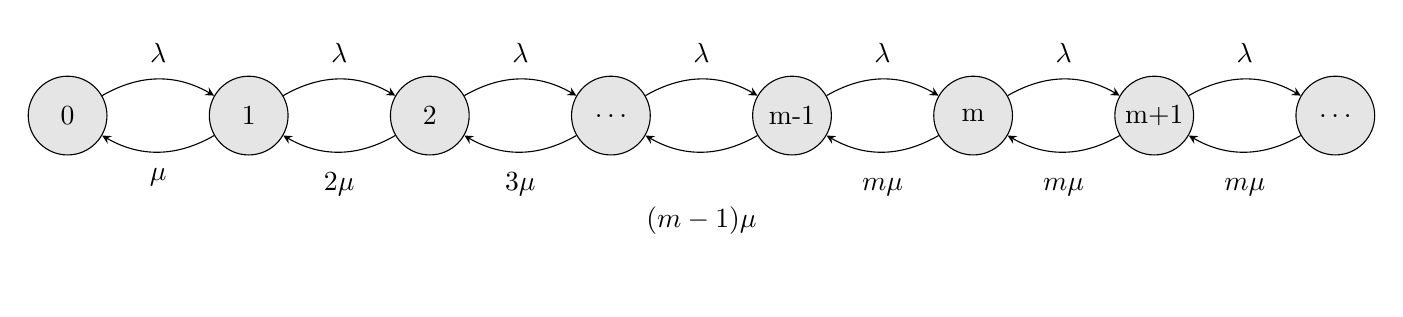
\begin{tikzpicture}[>=stealth, node distance=2.3cm, every node/.style={circle}]
    % Nodes
    \node (0) [{draw, fill=gray!20, minimum size=10mm, inner sep=0pt}] {0};
    \node (1) [{right of=0, draw, fill=gray!20, minimum size=10mm, inner sep=0pt}] {1};
    \node (2) [{right of=1, draw, fill=gray!20, minimum size=10mm, inner sep=0pt}] {2};
    \node (dots1) [{right of=2, draw, fill=gray!20, minimum size=10mm, inner sep=0pt}] {$\dots$};
    \node (m1) [{right of=dots1, draw, fill=gray!20, minimum size=10mm, inner sep=0pt}] {m-1};
    \node (m2) [{right of=m1, draw, fill=gray!20, minimum size=10mm, inner sep=0pt}] {m};
    \node (m3) [{right of=m2, draw, fill=gray!20, minimum size=10mm, inner sep=0pt}] {m+1};
    \node (dots2) [{right of=m3, draw, fill=gray!20, minimum size=10mm, inner sep=0pt}] {$\dots$};
  
  

    % Transition arrows for arrivals
    \draw[->] (0) to[bend left] node[above] {$\lambda$} (1);
    \draw[->] (1) to[bend left] node[above] {$\lambda$} (2);
    \draw[->] (2) to[bend left] node[above] {$\lambda$} (dots1);
    \draw[->] (dots1) to[bend left] node[above] {$\lambda$} (m1);
    \draw[->] (m1) to[bend left] node[above] {$\lambda$} (m2);
    \draw[->] (m2) to[bend left] node[above] {$\lambda$} (m3);
    \draw[->] (m3) to[bend left] node[above] {$\lambda$} (dots2);


    % Transition arrows for departures
    \draw[->] (1) to[bend left] node[below] {$\mu$} (0);
    \draw[->] (2) to[bend left] node[below] {$2\mu$} (1);
    \draw[->] (dots1) to[bend left] node[below] {$3\mu$} (2);
    \draw[->] (m1) to[bend left] node[below] {$(m-1)\mu$} (dots1);
    \draw[->] (m2) to[bend left] node[below] {$m \mu$} (m1);
    \draw[->] (m3) to[bend left] node[below] {$m \mu$} (m2);
    \draw[->] (dots2) to[bend left] node[below] {$m \mu$} (m3);

\end{tikzpicture}
